\documentclass[9pt,a4paper]{article}

% --- Fonts / encoding ---
\usepackage[utf8]{inputenc}
\usepackage[T1]{fontenc}
\usepackage{lmodern}            % scalable CM fonts
\usepackage{inconsolata}        % scalable \ttfamily for listings (avoids microtype issues)

% --- Layout & columns ---
\usepackage{geometry}
\geometry{margin=10mm}
\usepackage{multicol}
\setlength\columnsep{6mm}
\setlength\parskip{0pt}
\setlength\parindent{0pt}
\raggedbottom

% --- Typesetting helpers ---
\usepackage[final]{microtype}
\usepackage{enumitem}
\setlist[itemize]{left=1.2em,noitemsep,topsep=1pt}
\setlist[enumerate]{left=1.4em,noitemsep,topsep=1pt}
\usepackage{booktabs,tabularx}
\usepackage{amsmath,amssymb,mathtools}
\usepackage{hyperref}
\usepackage{array}
\usepackage{relsize}
\usepackage{bm}

% --- Code-like algorithms (very compact) ---
\usepackage{listings}
\lstdefinestyle{tight}{
  basicstyle=\ttfamily\footnotesize,
  numbers=none,numbersep=2pt,
  aboveskip=2pt,belowskip=2pt,
  xleftmargin=0pt,frame=single,framerule=0.2pt,
  framesep=2pt,columns=fullflexible,keepspaces=true,
  showstringspaces=false,breaklines=true,breakatwhitespace=true
}

% --- TikZ for schemas ---
\usepackage{tikz}
\usetikzlibrary{positioning,calc,trees}
\tikzset{
  smallnode/.style={circle,draw,inner sep=0.8pt,minimum size=9pt},
  smallrect/.style={rectangle,draw,inner sep=1.5pt},
  level distance/.initial=9mm
}

% --- Macros ---
\newcommand{\bigO}{\mathcal{O}}
\newcommand{\sect}[1]{\vspace{1ex}\textbf{\large #1}\par\vspace{0.3ex}\hrule\vspace{0.6ex}}
\newcommand{\subsect}[1]{\vspace{0.4ex}\textbf{#1}\par}

\begin{document}
\scriptsize

% ==================== PAGE 1 ====================
\begin{multicols}{3}
    \sloppy\raggedcolumns

    % =========================================================
    \sect{Recherche séquentielle}
    \textbf{Idée.} Balayer le tableau jusqu'à trouver $x$.
    \begin{lstlisting}[style=tight]
bool trouve=false; int i=0;
while (i<n && !trouve) {
  if (T[i]==x) trouve=true; else i++;
}
return trouve;
\end{lstlisting}
    \textbf{Complexité :} pire/moyenne $\bigO(n)$, meilleur $\bigO(1)$ si $x$ en tête.

    \subsect{Recherche dichotomique (binaire)}
    \emph{Précondition :} tableau trié.
    \begin{lstlisting}[style=tight]
int g=0, d=n-1;
while (g<=d){
  int m=(g+d)/2;
  if (T[m]==x) return true;
  if (T[m]<x) g=m+1; else d=m-1;
}
return false;
\end{lstlisting}
    \textbf{Complexité :} $\bigO(\log n)$.

    \subsect{Tableau vs. Liste chaînée}
    \begin{tabularx}{\linewidth}{@{}>{\bfseries}lX@{}}
        Tableau       & Accès aléatoire $\bigO(1)$, taille fixe                    \\
        Liste chaînée & Insertion/suppression en tête $\bigO(1)$, accès séquentiel \\
    \end{tabularx}

    \subsect{Piles et files}
    \begin{tabularx}{\linewidth}{@{}lX@{}}
        \textbf{Pile (LIFO)} &
        \begin{itemize}
            \item \textit{Tableau}: push/pop en fin $\bigO(1)$ amorti
            \item \textit{Liste}: push/pop en tête $\bigO(1)$
        \end{itemize} \\
        \textbf{File (FIFO)} &
        \begin{itemize}
            \item \textit{Tableau}: deux indices (tête/fin), opérations $\bigO(1)$
            \item \textit{Liste}: pointeur de fin, enq/deq $\bigO(1)$
        \end{itemize} \\
    \end{tabularx}

    % =========================================================
    \sect{Arbres}
    \textbf{Déf.} Nœud racine et sous-arbres (éventuellement vides).\\
    \textbf{Parcours} :
    préordre (racine, $A_g$, $A_d$),
    infixe ($A_g$, racine, $A_d$),
    postordre ($A_g$, $A_d$, racine).\\
    \textbf{Hauteur $h$ (nœuds $n$) :} $\lfloor\log_2 n\rfloor \le h \le n-1$.

    \subsect{Schéma AB (ex.)}
    \begin{center}
        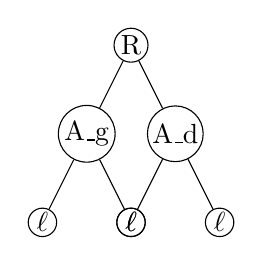
\begin{tikzpicture}[scale=0.75]
            \node[smallnode]{R}
            child{node[smallnode]{A\_g}
                    child{node[smallnode]{\(\ell\)}}
                    child{node[smallnode]{\(\ell\)}}
                }
            child{node[smallnode]{A\_d}
                    child{node[smallnode]{\(\ell\)}}
                    child{node[smallnode]{\(\ell\)}}
                };
        \end{tikzpicture}
    \end{center}

    \subsect{Tri : borne inférieure}
    Tout tri par comparaisons $\Rightarrow \Omega(n\log n)$ au pire.

    % =========================================================
    \sect{Tri par sélection}
    \textbf{Principe :} mettre le plus petit au début à chaque passe.
    \begin{lstlisting}[style=tight]
for (i=1..n-1){
  k=i;
  for (j=i+1..n) if (T[j]<T[k]) k=j;
  swap(T[i],T[k]);
}
\end{lstlisting}
    \textbf{Complexité :} $\bigO(n^2)$ (pire/moyen/meilleur).

    \subsect{Tri par insertion}
    Insérer $T[i]$ dans le préfixe trié.
    \begin{lstlisting}[style=tight]
for (i=2..n){
  x=T[i]; j=i-1;
  while (j>=1 && T[j]>x){ T[j+1]=T[j]; j--; }
  T[j+1]=x;
}
\end{lstlisting}
    \textbf{Complexité :} pire $\bigO(n^2)$, meilleur $\bigO(n)$.

    \subsect{Tri rapide (Quicksort)}
    Partitionner \& trier récursivement.
    \begin{lstlisting}[style=tight]
q = partition(T,l,r);
quicksort(T,l,q-1); quicksort(T,q+1,r);
\end{lstlisting}
    \textbf{Complexité :} moyenne $\bigO(n\log n)$, pire $\bigO(n^2)$.

    \subsect{Tri par ABR}
    Insérer dans un ABR puis parcours infixe $\Rightarrow$ séquence triée.\\
    Construction moyenne $\bigO(n\log n)$ (pire $\bigO(n^2)$), parcours $\bigO(n)$.

    % =========================================================
    \sect{Tas (Heap)}
    \subsect{Représentation tableau}
    Indices $1..n$ : gauche$(i)=2i$, droite$(i)=2i+1$, parent$(i)=\lfloor i/2\rfloor$.

    \subsect{Schéma de tas}
    \begin{center}
        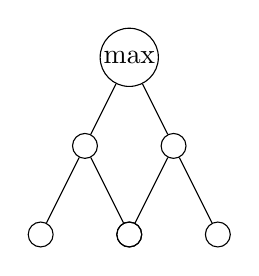
\begin{tikzpicture}[scale=0.75]
            \node[smallnode]{\(\max\)}
            child{node[smallnode]{}
                    child{node[smallnode]{}}
                    child{node[smallnode]{}}
                }
            child{node[smallnode]{}
                    child{node[smallnode]{}}
                    child{node[smallnode]{}}
                };
        \end{tikzpicture}
    \end{center}

    \textbf{Opérations :} \emph{heapify} $\bigO(\log n)$,
    build-heap $\bigO(n)$, insertion/extract-max $\bigO(\log n)$.\\
    \textbf{Tri par tas :} $\bigO(n\log n)$.

    % =========================================================
    \sect{Hachage}
    \textbf{But :} appartenance de mots dans une table $m$ cases.\\
    Fonction $h:U\to\{0,\dots,m-1\}$, facteur de charge $\alpha=n/m$.\\
    \textbf{Chaînage :} coût attendu $\bigO(1+\alpha)$ pour recherche/insertion; pire $\bigO(n)$.

    \subsect{Principe de recherche}
    \begin{enumerate}
        \item Calculer $i=h(x)$
        \item Parcourir la liste du seau $i$
        \item Trouvé $\Rightarrow$ succès sinon échec
    \end{enumerate}

    \subsect{Gestion des collisions}
    \begin{itemize}
        \item Listes chaînées par seau
        \item Adressage ouvert (linéaire, quadratique, double hachage)
    \end{itemize}

    % =========================================================
    \sect{Algorithme de Huffman}
    \textbf{Objectif :} code préfixe minimisant $L=\sum_c \mathrm{occ}(c)\,\ell(c)$. \\
    \textbf{Construction :} file de priorité fusionnant toujours les 2 plus petites fréquences.\\
    \textbf{Complexité :} $\bigO(k\log k)$ pour $k$ caractères.

    \subsect{Schéma (exemple)}
    \begin{center}
        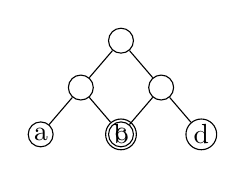
\begin{tikzpicture}[level distance=7mm, sibling distance=12mm, scale=0.85]
            \node[smallnode]{}
            child{ node[smallnode]{}
                    child{ node[smallnode]{a} }
                    child{ node[smallnode]{b} }
                }
            child{ node[smallnode]{}
                    child{ node[smallnode]{c} }
                    child{ node[smallnode]{d} }
                };
        \end{tikzpicture}
    \end{center}
    \emph{Propriété de préfixe :} aucun code n'est préfixe d'un autre.

    % =========================================================
    \sect{Récapitulatif des complexités}
    \begin{tabularx}{\linewidth}{@{}l>{\raggedleft\arraybackslash}X@{}}
        Recherche séquentielle & $\bigO(n)$                               \\
        Recherche binaire      & $\bigO(\log n)$                          \\
        Tri sélection          & $\bigO(n^2)$                             \\
        Tri insertion          & pire $\bigO(n^2)$, meilleur $\bigO(n)$   \\
        Quicksort              & moy. $\bigO(n\log n)$, pire $\bigO(n^2)$ \\
        Tri par tas            & $\bigO(n\log n)$                         \\
        Tri via ABR            & moy. $\bigO(n\log n)$, pire $\bigO(n^2)$ \\
        Tas (build / op.)      & $\bigO(n)$ / $\bigO(\log n)$             \\
        Hachage (attendu)      & $\bigO(1)$ par op. si $\alpha$ borné     \\
        Huffman                & $\bigO(k\log k)$                         \\
    \end{tabularx}

\end{multicols}

% ==================== PAGE 2 ====================
\newpage
\begin{multicols}{3}
    \sloppy\raggedcolumns
    \scriptsize

    \sect{Graphes (orientation, bases)}
    \textbf{Graphe fini simple orienté :} $G=(X,A)$, $X$ ensemble fini de sommets, $A\subseteq X\times X$ sans boucle ni multi-arcs.\\
    \textbf{Degrés :} $\deg^+(x)=|\{(x,y)\in A\}|,\;\deg^-(x)=|\{(y,x)\in A\}|.$
    \[
        n=|X|,\qquad m=|A|,\qquad \sum_{x\in X}\deg^+(x)=\sum_{x\in X}\deg^-(x)=m.
    \]
    \textbf{Chaîne (chemin)} : $(x_0,\ldots,x_k)$ avec $(x_i,x_{i+1})\in A$.\\
    \textbf{Simple} : pas de sommet répété; \textbf{circuit} : $x_0=x_k$; \textbf{élémentaire} : simple et sans répétition d’arcs.\\
    \textbf{Fortement connexe :} $\forall x,y$ chaîne de $x$ vers $y$. \\
    \textbf{Composante fortement connexe (CFC)} : classe d’équivalence par la relation “$x\leadsto y$ et $y\leadsto x$”.

    \subsect{Partition en CFC}
    Soient $C_1,\ldots,C_k$ les CFC de $G$ :
    \begin{enumerate}
        \item $X=\bigsqcup_{i=1}^k C_i$
        \item Si $i\ne j$, $C_i\cap C_j=\varnothing$
        \item Le graphe des CFC (condensation) est un DAG.
    \end{enumerate}

    \subsect{Représentations}
    \textbf{Matrice d’adjacence} $M=(m_{xy})$ avec $m_{xy}=1$ si $(x,y)\in A$, sinon $0$.\\
    \textbf{Listes d’adjacence :} pour chaque $x$, la liste de ses successeurs (ou prédécesseurs). \\
    \textbf{Coût mémoire :} matrice $\Theta(n^2)$, listes $\Theta(n+m)$.

    \sect{Plus court \& plus long chemin}
    \textbf{Plus court chemin (pcc).} Longueur = somme des poids $w(a)$.\\
    \textbf{Absorbant (négatif) :} un circuit de poids $<0$ $\Rightarrow$ pas de pcc.\\
    \textbf{Plus long chemin.} NP-difficile en général; dans un DAG on peut le faire en ordre topologique (changer $\min\to\max$).

    \subsect{Dijkstra ($w\ge 0$)}
    \textbf{Hyp.} poids non négatifs. \textbf{Idée :} invariant d’ensemble $S$ des sommets “figés”.
    \begin{lstlisting}[style=tight]
Init:  d[s]=0; d[x]=+inf pour x!=s; S={}
Tant que S!=X:
  u = argmin_{x in X\S} d[x]
  S = S U {u}
  pour (u,v) in A:
    si d[v] > d[u] + w(u,v):
       d[v] = d[u] + w(u,v); pere[v]=u
\end{lstlisting}
    \textbf{Complexité :} $\bigO(n^2)$ avec matrice; $\bigO((n+m)\log n)$ avec tas binaire.

    \subsect{Bellman-Ford (poids quelconques)}
    Détecte circuits négatifs; calcule les pcc si aucun accessible à $s$.
    \begin{lstlisting}[style=tight]
Init: d[s]=0, d[x]=+inf sinon
Repeter n-1 fois:
  pour chaque arc (u,v):
    d[v] = min(d[v], d[u] + w(u,v))
Verif circuit negatif:
  s'il existe (u,v) avec d[v] > d[u] + w(u,v) -> negatif
\end{lstlisting}
    \textbf{Complexité :} $\bigO(n\,m)$.

    \sect{Graphe sans circuit (DAG)}
    \subsect{Numérotation/ordre topologique}
    \textbf{Déf.} Bijection $\tau:X\to\{1,\dots,n\}$ telle que $(x,y)\in A \Rightarrow \tau(x)<\tau(y)$. \\
    \textbf{Propriété :} $G$ est un DAG $\Leftrightarrow$ un ordre topologique existe.

    \subsect{Calcul d’un ordre topo (Kahn)}
    \begin{lstlisting}[style=tight]
Entree: DAG G
S = {sommmets d'indegre 0}; ordre=[]
Tant que S non vide:
  u = extraire(S)
  ordre.ajouter(u)
  pour (u,v) in A:
    enlever (u,v); si indegre(v)==0: S.ajouter(v)
\end{lstlisting}
    \textbf{Complexité :} $\bigO(n+m)$.

    \subsect{Pcc dans un DAG (Bellman “topo”)}
    \begin{lstlisting}[style=tight]
Entree: DAG, ordre topologique t(1..n)
Init d[s]=0; d[x]=+inf sinon; pere[x]=nil
Pour i=1..n (dans l'ordre topo):
  u = t[i]
  pour (u,v) in A:
    si d[v] > d[u] + w(u,v):
       d[v] = d[u] + w(u,v); pere[v]=u
\end{lstlisting}
    \textbf{Complexité :} $\bigO(n+m)$.

    \sect{Graphe non orienté}
    Arêtes non ordonnées $\{x,y\}$. \quad $G=(X,E)$, $n=|X|$, $m=|E|$.\\
    \textbf{Degré} $d(x)$ nombre d’arêtes incidentes à $x$.
    \[
        \sum_{x\in X} d(x)=2m \quad \text{(handshaking)}.
    \]
    \textbf{Chaîne} : $(x_0,\ldots,x_k)$ avec $\{x_i,x_{i+1}\}\in E$. \\
    \textbf{Cycle} : $x_0=x_k$, $k\ge 3$. \\
    \textbf{Connexité} : $\forall x,y$ chaîne entre $x$ et $y$. Les composantes connexes $C_1,\dots,C_r$ partitionnent $X$.\\
    \textbf{Forêt/Arbre couvrant :} sous-graphe $(X,F)$, acyclique, connexe, $|F|=n-1$.\\
    \textbf{Pont (arête isthme)} : arête dont la suppression augmente le nombre de composantes.

    \subsect{Conséquences}
    \begin{itemize}
        \item Si $G$ est connexe, alors $m\ge n-1$.
        \item $G$ connexe $\Rightarrow$ il existe un arbre couvrant.
        \item Un cycle $\Rightarrow$ on peut retirer une arête du cycle sans perdre la connexité.
    \end{itemize}

    \sect{Utilisation typique (pères \& distances)}
    Soit un parcours (BFS/DFS) depuis $s$. On enregistre $d(x)$ (distance/numéro) et $p(x)$ (père).
    \begin{center}
        \begin{tabular}{r|c|c}
            $x$      & $d(x)$   & $p(x)$   \\\hline
            $s$      & $0$      & --       \\
            $\cdots$ & $\cdots$ & $\cdots$
        \end{tabular}
    \end{center}
    \textbf{Propriété (BFS) :} si $G$ non pondéré (ou poids $1$), $d(x)$ est la longueur du pcc $s\leadsto x$ et l’arbre des pères est un arbre des plus courts chemins.

    \sect{Remarques pratiques}
    \begin{itemize}
        \item \textbf{Choix de structure :} matrice pour graphes denses; listes pour graphes clairsemés.
        \item \textbf{Chemins longs/courts dans DAG :} même DP sur ordre topo avec $\max$ ou $\min$.
        \item \textbf{Détection de cycles :} un ordre topo n’existe pas $\Leftrightarrow$ il y a un cycle.
    \end{itemize}

\end{multicols}

% ==================== PAGE 3 ====================
\newpage
\begin{multicols}{3}
    \sloppy\raggedcolumns
    \scriptsize

    \sect{Lemmes et THM (graphes non orientés)}
    \textbf{Lemme 2.} Si $G$ est sans cycle alors $m\le n-1$. \quad
    \textbf{Corollaire.} Un arbre a $n$ sommets, $n-1$ arêtes.\\
    \textbf{Lemme 3.} $a\in E$ est un isthme $\Leftrightarrow$ $a$ n'appartient à \emph{aucun} cycle.\\
    \textbf{THM équivalences pour $G$ connexe} :
    \begin{enumerate}
        \item $G$ connexe et $m=n-1$
        \item $G$ est sans cycle
        \item Il existe une unique chaîne simple entre $x$ et $y$ pour tout $x\neq y$
        \item $G$ est connexe et l'ajout d'une arête crée un cycle
    \end{enumerate}

    \sect{Algorithme de Kruskal (ACM poids min)}
    \textbf{Principe.}
    \begin{enumerate}
        \item Trier les arêtes par poids croissant
        \item Parcourir la liste et ajouter l'arête si elle ne crée pas de cycle
    \end{enumerate}
    \textbf{Test de cycle :} union-find (composantes).\\
    \textbf{Pseudo-code (schéma).}
    \begin{lstlisting}[style=tight]
ACM = {}
trier E par poids croissant
pour (u,v) dans E:
  if find(u)!=find(v):
     ACM.add((u,v)); union(u,v)
\end{lstlisting}
    \textbf{Complexité :} $\bigO(m\log m)$ (tri) $+\bigO(m\,\alpha(n))$ (UF).

    \subsect{Détection de cycle par CC (version simple)}
    On maintient $CC[i]$ = numéro de composante du sommet $i$; fusion si arête choisie.\\
    \textbf{Complexité illustrée :} $\bigO(m \log m)+n^2$ (naïf).

    \sect{Algorithme de Prim (ACM)}
    \textbf{Principe.} Démarre d'un sommet; à chaque étape, ajoute l'arête la moins chère incidente à l'arbre courant.
    \begin{lstlisting}[style=tight]
S = {s};  poids[v]=+inf; pere[v]=nil
maj voisins de s
tant que |S|<n:
  u = argmin_{v notin S} poids[v]
  S = S U {u}
  pour (u,w) arete:
    si w notin S et c(u,w) < poids[w]:
       poids[w]=c(u,w); pere[w]=u
\end{lstlisting}
    \textbf{Complexité :} $\bigO(n^2)$ (matrice), $\bigO(m\log n)$ (tas binaire).

    \sect{Parcours d'un graphe}
    \subsect{Parcours orienté (schéma ``marquer/examiner'')}
    \begin{itemize}
        \item Au départ, aucun sommet marqué; aucune arête traversée
        \item Choisir un sommet $x$; \textbf{traverser} $(x,y)$ si non traversée
        \item Si $y$ non marqué $\Rightarrow$ marquer $y$, $père(y)=x$
    \end{itemize}
    Boucle sur les arêtes jusqu'à ce que tous les sommets soient examinés.\\
    \textbf{Coût :} $\bigO(n+m)$.

    \subsect{Parcours non orienté}
    Même idée avec arêtes $\{x,y\}$; les composantes connexes émergent naturellement.

    \sect{BFS (largeur) \& DFS (profondeur)}
    \subsect{BFS (file)}
    \begin{lstlisting}[style=tight]
marquer s; d[s]=0; Q={s}
while Q non vide:
  u=dequeue(Q)
  pour (u,v):
    si v non marque:
      marquer v; d[v]=d[u]+1; pere[v]=u; enqueue(Q,v)
\end{lstlisting}
    \textbf{Propriété.} $d[v]=$ distance minimale (non pondéré). \quad \textbf{Complexité.} $\bigO(n+m)$.

    \subsect{DFS (pile/récursif)}
    \begin{lstlisting}[style=tight]
DFS(u):
  pre[u]=++time
  pour (u,v):
    si v non visite: pere[v]=u; DFS(v)
  post[u]=++time
\end{lstlisting}
    \textbf{Numérotations pré/postfixe.} $pre[u]$ à l'entrée, $post[u]$ à la sortie. Utile pour CFC/topo.

    \sect{CFC (composantes fortement connexes)}
    \textbf{Kosaraju (2 DFS).}
    \begin{enumerate}
        \item DFS sur $G$ pour obtenir l'ordre décroissant de $post$.
        \item DFS sur $G^{T}$ en suivant cet ordre; chaque arbre découvert $\Rightarrow$ une CFC.
    \end{enumerate}
    \textbf{Complexité :} $\bigO(n+m)$.

    \sect{Flot maximum \& coupe minimum}
    \textbf{Réseau.} $G=(X,A)$ orienté valué par capacités $c:A\to\mathbb{R}_+$; source $s$, puits $t$.\\
    \textbf{Flot.} $f:A\to\mathbb{R}$ tel que :
    \begin{itemize}
        \item (Capacité) $0\le f(x,y)\le c(x,y)$
        \item (Conservation) $\sum_y f(y,x)=\sum_y f(x,y)$ pour $x\neq s,t$
    \end{itemize}
    \textbf{Valeur.} $|f|=\sum_y f(s,y)-\sum_y f(y,s)$.\\
    \textbf{Résiduel.} $c_f(x,y)=c(x,y)-f(x,y)$ et arc retour $(y,x)$ de capacité $f(x,y)$.

    \subsect{Théorème (Max-flow / Min-cut)}
    Pour tout flot $f$ et toute coupe $(S,\bar S)$ avec $s\in S$, $t\in \bar S$ :
    \[
        |f| \le c(S,\bar S)=\sum_{x\in S,\,y\in\bar S} c(x,y),
    \]
    avec égalité $\Leftrightarrow$ $f$ est maximum et la coupe est minimum.

    \sect{Ford--Fulkerson (chemins augmentants)}
    \textbf{Idée.}
    \begin{enumerate}
        \item Initialiser $f=0$; calculer le résiduel $G_f$
        \item Tant qu'il existe un chemin $P$ de $s$ à $t$ dans $G_f$:
        \item \quad $\Delta=\min\{c_f(e): e\in P\}$; augmenter $f$ de $\Delta$ le long de $P$
    \end{enumerate}
    \textbf{Complexité.} Dépend du choix des chemins. Avec BFS (Edmonds--Karp) : $\bigO(n\,m^2)$.\\
    \textbf{Arrêt.} Aucun chemin augmentant $\Rightarrow$ flot max atteint; les sommets atteignables dans $G_f$ définissent une coupe min.

    \sect{Notes rapides \& rappels}
    \begin{itemize}
        \item \textbf{Pont/isthme.} Suppression augmente le \# de composantes.
        \item \textbf{Arbre couvrant.} $n-1$ arêtes; unique chemin simple entre deux sommets.
        \item \textbf{DAG.} Numérotation topologique $\Leftrightarrow$ pas de cycle.
        \item \textbf{Choix structures.} Matrice $\Theta(n^2)$ (dense), listes $\Theta(n+m)$ (sparse).
        \item \textbf{Coûts typiques.} BFS/DFS $\bigO(n+m)$; Kruskal $\bigO(m\log n)$; Prim $\bigO(m\log n)$; CFC $\bigO(n+m)$; Edmonds--Karp $\bigO(n m^2)$.
    \end{itemize}

\end{multicols}

% ==================== PAGE 4 (TRANSCRIPTION DE L'IMAGE) ====================
\newpage
\begin{multicols}{3}
    \sloppy\raggedcolumns
    \scriptsize

    \sect{Coupes, marquages et flot}
    \textbf{Coupe $(S,\bar S)$.} $s\in S$, $t\in\bar S$. Capacité $c(S,\bar S)=\sum_{x\in S,\,y\in\bar S}c(x,y)$. \\
    \textbf{Résiduel.} $c_f(x,y)=c(x,y)-f(x,y)$ (arc retour $(y,x)$ de capacité $f(x,y)$). \\
    \textbf{Algorithme de marquage (après arrêt).}
    \begin{itemize}
        \item Marquer $s$.
        \item Tant qu'il existe un sommet marqué $x$ et un voisin $y$ non marqué tel que
              \[
                  c_f(x,y)>0 \ \text{(arc direct disponible)} \quad\text{ou}\quad c_f(y,x)>0 \ \text{(arc retour)} ,
              \]
              marquer $y$.
    \end{itemize}
    À la fin, $S=\{$sommets marqués$\}$ : \emph{les arcs traversant de $S$ vers $\bar S$ sont saturés et ceux de $\bar S$ vers $S$ portent du flot nul}. $(S,\bar S)$ est une \textbf{coupe minimum} et $|f|=c(S,\bar S)$.

    \subsect{Ford--Fulkerson (rappel succinct)}
    \begin{lstlisting}[style=tight]
f=0; construire G_f
tant qu'il existe un chemin P de s a t dans G_f:
  Delta = min{ c_f(e) : e dans P }
  augmenter f de Delta le long de P
  mettre a jour G_f
\end{lstlisting}
    \textbf{Complexités usuelles.} FF naïf : peut être pseudo-polynomial. Edmonds--Karp (BFS dans $G_f$) : $\bigO(nm^2)$.

    \sect{Application : Couplage maximum biparti}
    Soit $G=(X\cup Y,E)$ biparti. Construire le réseau :
    \begin{itemize}
        \item arcs $s\to x$ ($x\in X$) de capacité $1$ ;
        \item arcs $x\to y$ pour $(x,y)\in E$ de capacité $1$ ;
        \item arcs $y\to t$ ($y\in Y$) de capacité $1$.
    \end{itemize}
    Tout flot $f$ correspond à un \textbf{couplage} $C=\{(x,y): f(x,y)=1\}$.
    Max-flot $=$ taille du couplage maximum. \\
    \textbf{Complexité (implémentation simple).} $\bigO(mn)$ ; avec Hopcroft--Karp : $\bigO(\sqrt{n}\,m)$.

    \sect{Théorème de Menger (version arcs)}
    Pour $a,b\in X$, soient $N_{a,b}$ le \# minimal d'arcs à supprimer pour séparer $a$ de $b$, et $P_{a,b}$ le \# maximal de \textbf{chemins arc-disjoints} de $a$ à $b$. Alors
    \[
        N_{a,b}=P_{a,b}.
    \]
    \textbf{Idée de preuve.} Réduction à un réseau : capacité $1$ par arc, max-flot $=$ \# de chemins arc-disjoints, min-coupe $=$ \# d'arcs à retirer. Donc $P_{a,b}=N_{a,b}$.

    \sect{Taille de codage \& problèmes de décision}
    Une \textbf{instance} $\mathbf{I}$ est encodée binaire; $\mathrm{taille}(\mathbf{I})=|\mathbf{I}|$ (en bits). \\
    Un \textbf{problème de décision} attend ``oui/non''. On dit qu'un algorithme est \textbf{polynomial} si son temps est majoré par $|\mathbf{I}|^k$ pour un $k$ constant.

    \subsect{Classes P et NP}
    \begin{itemize}
        \item \textbf{P} : problèmes décidables en temps polynomial.
        \item \textbf{NP} : ``vérifiables'' en temps polynômial : si la réponse est ``oui'', il existe un \textbf{certificat} $y$ de taille polynomiale vérifiable en $poly(|\mathbf{I}|)$.
    \end{itemize}
    On sait $P\subseteq NP$. On ignore si $P=NP$.

    \subsect{Réductions polynomiales}
    $\Pi_1 \le_P \Pi_2$ s'il existe une transformation polynomiale $T$ telle que
    \[
        \mathbf{I}\in \Pi_1 \iff T(\mathbf{I})\in \Pi_2 .
    \]
    Si $\Pi_1 \le_P \Pi_2$ et $\Pi_2$ est polynomiale, alors $\Pi_1$ l'est aussi.

    \subsect{NP-difficile / NP-complet}
    \begin{itemize}
        \item \textbf{NP-difficile} : tout problème de NP s'y réduit.
        \item \textbf{NP-complet} : dans NP \emph{et} NP-difficile.
    \end{itemize}

    \sect{Exemples classiques (NP-complétude)}
    \begin{itemize}
        \item \textbf{3-SAT} : formule CNF à clauses de taille $3$ satisfiable ?
        \item \textbf{PVC} (Vertex Cover) : existe-t-il $k$ sommets couvrant toutes les arêtes ?
        \item \textbf{Stable/IS} : existe-t-il un ensemble stable (indépendant) de taille $\ge k$ ?
        \item \textbf{Clique} : existe-t-il une clique de taille $\ge k$ ?
    \end{itemize}
    Chaîne de réductions standard :
    \[
        \text{3-SAT} \;\le_P\; \text{Clique} \;\equiv_P\; \text{Stable} \;\le_P\; \text{PVC}.
    \]
    Donc \textbf{PVC}, \textbf{Stable} et \textbf{Clique} sont NP-complets (et de même pour 3-SAT).

    \sect{Complexité de quelques algorithmes de flots}
    \begin{tabularx}{\linewidth}{@{}l>{\raggedleft\arraybackslash}X@{}}
        Ford--Fulkerson (chemins arbitraires) & pseudo-polynomial  \\
        Edmonds--Karp (BFS)                   & $\bigO(n m^2)$     \\
        Dinic (niveaux + blocs)               & $\bigO(n^2 m)$     \\
        Biparti (Hopcroft--Karp)              & $\bigO(m\sqrt{n})$ \\
    \end{tabularx}

    \sect{Notes rapides de cours}
    \begin{itemize}
        \item Dans la coupe min issue du marquage, \emph{les arcs retenus par la forte $a$-$b$-connexité} sont ceux franchissant $S\to\bar S$.
        \item Pour numéroter un DAG, on peut numéroter de $1$ à $n$ en suivant l'ordre topologique.
        \item Les tableaux de pères/distances (BFS/DFS) suffisent à reconstruire des chemins.
    \end{itemize}

\end{multicols}

\end{document}
